\section{Identification of existing tools}
Every day, Cisco - in collaboration with Shadow \cite{shadow} - drops a ZIP archive containing about a thousand malware on a server. Once extracted, we get the binary of each malware as well as its corresponding hash used as its filename. Unfortunately, we do not have any additional information regarding these files. The main objective is to identify whether they have been packed. Once each piece of malware is labeled as \textit{packed} or \textit{not packed}, we will be able to use them in our learning algorithms.

After investigation, we discovered several software that can extract various information out of a binary file, including its packer, if any. However, we have no guarantee about their accuracy, so we will compare them and gather the ones having distinct methods of operation. Indeed, if they all agree to identify a specific packer for a malware using different techniques, they are more likely to be right.

We identified 14 different detectors, listed in table \ref{Tab:list_detectors}. Each detector is different and has its own characteristics. However, some of them share common features. Below, we describe the five categories we came up with in order to provide a clearer classification.

\begin{itemize}
    \item \textbf{GitHub :} Allows to indicate whether the software is available on the platform. By reading the source code of the detector, we can understand how it works and determine if it is, thanks to the latest commits, still up-to-date. Moreover, the number of \textbf{stars} gives a rough idea of its popularity among the GitHub community. As an example, the detectors RetDec and Detect-it-Easy count 5 400 and 1 500 of them respectively.
    \item \textbf{Use :} Divided in two groups based on the way the detector extracts information related to the packers.
        \begin{enumerate}
            \item \textbf{PEiD-like:} The PEiD software uses a database called \textit{userdb.txt} which contains several signatures of the first entry point bytes of malware packed with a certain packer. Once a new malware is analysed, PEiD compares its signature with the ones from the database in order to find the corresponding packer.
            
            As an example, the following signature allows to identify malware packed with the version 3 of the Borland Delphi packer. The \texttt{??} symbols correspond to wildcards.
            
{\noindent\begin{lstlisting}
[Borland Delphi v3.0]
signature = 50 6A ?? E8 ?? ?? FF FF BA ?? ?? ?? ?? 52 89 05 ?? ?? ?? ?? 89 42 04 E8 ?? ?? ?? ?? 5A 58 E8 ?? ?? ?? ?? C3 55 8B EC 33 C0
ep_only = true
\end{lstlisting}}
            Software based on the same technique are tagged as \textbf{peid}. Most of the time, they even use the same database.
            \item \textbf{Yara rules:} Such rules are widely used in malware analysis. In this case, one Yara rule identifies a packer and consists of a set of static filters that the detector will scan when analysing a new binary. Regarding the number of matches, the detector will decide whether the file was packed with the specific packer.
        \end{enumerate}
    \item \textbf{OS :} The operating system on which the detector operates, namely Windows, Linux or macOS.
    \item \textbf{Control :} Indicates if the software offers a command line interface (CLI), a graphical user interface (GUI) or both.
    \item \textbf{Maintained :} Tells if the detector is regularly maintained in 2020. For example, the software Language 2000 was not updated since 2000 while Detect-it-Easy receives daily updates.
\end{itemize}

\begin{table}[H]
\centering
\begin{tabular}{|l|c|c|c|c|c|}
    \hline
    \textbf{Name} & \textbf{GitHub} & \textbf{Use} & \textbf{OS} & \textbf{Control} & \textbf{Maintained}  \\
    \hline \hline
    AnalyzePe & Yes & peid & Cross-platform & CLI & No \\
    Detect-it-Easy & Yes & Yara & Cross-platform & Both & Yes \\
    ExeInfo Pe & No & peid & Windows & GUI & Yes \\
    ExeScan & Yes & peid & Cross-platform & CLI & No \\
    Language 2000 & No & ? & Windows & GUI & No \\
    Manalyze & Yes & Yara & Linux/Windows & CLI & Yes \\
    Nauz & Yes & ? & Cross-platform & Both & Yes \\ 
    Pe-bear & No & ? & Linux/Windows & Both & Yes \\
    PEiD & No & peid & Windows & GUI & No \\
    PEframe & Yes & Yara & Cross-platform & CLI & Yes \\ 
    PortEx & Yes & peid & Cross-platform & GUI & No \\
    Q-Unpack & Yes & ? & Cross-platform & CLI & No \\
    RetDet & Yes & Yara & Cross-platform & CLI & Yes \\
    RDG & No & peid & Windows & GUI & No \\
    \hline
\end{tabular}
\caption{Listing of the identified detectors}
\label{Tab:list_detectors}
\end{table}

One detector is missing in the table, namely the software created by Cisco and used by Biondi et al. \cite{biondi_effective_2019}. The reason is that although we are granted access to this tool, we are not aware of how it actually works. The system used to get the results of their analysis operates like a black-box: hash values of the malware we want to analyse are sent to Cisco via a text file, they proceed to their analysis and then send us back another text file with the corresponding results. Nevertheless, this detector is considered in further sections but because of its functioning, we are not able to categorise it in the above table.

\section{Evaluation of identified software}

When comparing the value returned by these static detectors over the same malware, it appeared that they did not always return the same output. While sometimes they just did not recognise the same packer, it also happened that they did not agree if the binary was packed or not. Therefore, the goal of this section is to design a system that combines several outputs to improve the overall accuracy. Moreover, we want to provide a more reliable prediction per malware by imposing an acceptance threshold. For example, a malware would be considered as packed when more than 60\% of the detectors say it is. 

Ideally, this new "super" detector should use as many software as possible among the ones found in the previous section in order to increase its accuracy. However, we should be careful not to use several times those working in the same way, otherwise it would considerably increase their weights in the decision process. As we receive new data on a daily basis, our fully automated detector should also be able to extract and analyse data continuously and without any human intervention. Moreover, the tool should be as modular as possible so that we can easily update and extend it with new detectors, new malware or new features. Finally, it should perform as quickly as possible to analyse as much malware as possible. Indeed, the larger the dataset, the more data we can give to the learning algorithms and the more powerful they should become.

\subsection{Graphical User Interface (GUI)}

We started by trying to automate the packing detection software that only worked through graphical user interfaces. The PyAutoGUI Python library \cite{pyautogui} allows to simulate keyboard inputs as well as mouse movements. To move the cursor in an automated fashion, there are two different options. The first possibility is to consider the screen as a Cartesian plane in which the mouse is given a starting point thanks to \textit{(x,y)} coordinates. To perform further movements, other instructions with distances expressed in pixels need to be provided. A typical scenario would be to ask the cursor to move 100 pixels to the right from its current location, then 500 pixels down, right click on the actual location and perform a copy. Some optimisations are also available, such as using keyboard shortcuts instead of a sequence of clicks and moves. The second method requires to take screenshots of specific areas beforehand, and then ask the cursor to teleport itself to the position matching the content of the picture.

Although the library worked relatively well for mouse movements, there were some problems regarding text insertions. We tried to use the \texttt{write()} function from PyAutoGUI for text insertion and to simulate key inputs one by one, but in both cases the text displayed did not match what we had typed. Eventually, the only trick that worked was to copy the text into the clipboard and then pasting it in the desired area.

In order for this automation system to work properly, we had to add a small delay between each instruction. If not, some operations did not have enough time to be performed and were simply skipped. This significantly slowed down the whole process. In addition, we had to let the graphical interface run continuously on the computer, without ever being able to perform any another tasks since both the keyboard and the mouse were used. All this together, we realised that this automation technique was really cumbersome and time consuming. We eventually decided to set this technique aside at that point.

\subsection{Command Line Interface (CLI)}

Despite the fact that Detect-it-Easy only provides a graphical version for Windows and macOS, a Linux archive exists, containing a lightweight and a command line version of this tool. Similarly, we can extract the database used by PEiD and exploit it thanks to a Python library called Pefile \cite{pefile}. This solution enables the creation of a command line and cross-platform alternative to PEiD.

Fortunately, the software already available via command lines are very easy to use. The malware is given as parameter and they directly output the result, i.e. if and how the binary was packed. Furthermore, almost all of them accept the option that allows to parse the output in \texttt{json} format, facilitating its further use.

\subsection{Management of multiple outputs}
During the execution of the PEframe detector, we were surprised when noticing that it provided more than one result per input file. Two hypotheses were put forward to justify such diverse outcomes :
\begin{enumerate}
    \item If a software was packed several times by the same packer or by different packers, PEframe can detect all of them.
    \item We know that most of the detections works by analysing whether certain portions of the binary file match certain predefined rules. If an executable matches several classification rules, the detector might doubt over its properties and return the different identified packers as a safety measure.
\end{enumerate}

To answer this question, we established three scenarios where a binary was packed with a packer A and then a packer B before given for analysis to PEframe :
\begin{enumerate}
    \item If we compressed the software with packer A and then with packer B, the detector only proclaimed packer B.
    \item When switching the packing order, packer A was detected.
    \item By using twice the same packer, saying A, PEframe found A only once.
\end{enumerate}

We observed that the detector can thus only identify the last packer used, which lets the question of multiple results unsolved. Therefore, we decided to manually check for a few binaries what these other outcomes were related to. After investigation, it turned out that they corresponded to broader information such as the linker, the compiler or the libraries used. Since they were not relevant for our packing detection problem, we did not considered them and eventually kept only the packer.

\section{Final selection of detectors}

We can not use all the detectors for our analysis. Firstly, although we found a way to automate GUI software, we cannot afford to leave our personal computers on and connected to the internet continuously. This issue can be solved by interacting with a Linux server through a SSH connection. We therefore need access to command line interfaces. Secondly, using all of them would not be feasible in terms of time. We tried to launch all detectors on the same malware and the overall process was impressively slow, mainly bounded by the most time consuming software. We hence had to make a selection. After consideration, we eventually decided to limit our solution to the following five detectors: 

\begin{itemize}
    \item \textbf{Cisco} We have the possibility to send them a list of malware - via their hash values - in order to get their analysis back. As aforementioned, we have no idea how this detector works but since we noticed that its results sometimes differed from the other detectors, we thought that it would be relevant to integrate it in our tool. Nevertheless, we are aware about the organisation such communication system requires. 
    \item \textbf{PEiD} \cite{peid} Although PEiD is no longer maintained, it remains the best-known and most widely used detector. We will only use its database which we will exploit via the Pefile library.
    \item \textbf{Detect-it-Easy} \cite{die} Also widely used, we chose this detector to maintain some diversity in methods since it works using Yara rules.
    \item \textbf{Manalyze} \cite{manalyze} This detector is mainly used by large companies. We were therefore curious to see if it would provide different outcomes.
    \item \textbf{PEframe} \cite{peframe} Since it works with Python, this software will be very easy to install, customise and automate. Given that in general it takes a bit more time than its peers, we infer that it might embed different detection mechanisms than the other detectors.
\end{itemize}

\subsection{Building the "super" detector}

In this section, we imagine a first version of our "super" detector. At first, it should be very simple : it takes a malware as input and displays the results of the four detectors selected in the previous section others than Cisco on the standard output. We do not consider Cisco here because we cannot run their tool directly and get an instant reply. Proceeding that way will already significantly enhance the analysis since we do not have to pass the file to each detector one by one anymore.

The class diagram (Figure \ref{fig:Detector}) confirms that this first version is very simple. We have one class per detector that extends \texttt{PackerDetector}, which acts as a parent and allows to have uniformity between the different tools. Each created class will take care, thanks to its \texttt{analyze()} method, of running the corresponding detector in a subprocess, get its output and reformat it. Formatting is necessary because, while some program return several results, like PEframe, in general the detectors do not issue the answer in the same format - additional text messages, date of the analysis, \texttt{json} format and so on. This step then ensures that all detectors simply deliver the name of the packer or \texttt{none} if the binary is not packed. Sometimes, a detector can fail to scan a malware for any reason. The \texttt{analyze()} method catches the exception and returns the \texttt{error} message instead of the packer name. 

\begin{figure}[hb]
\centering
  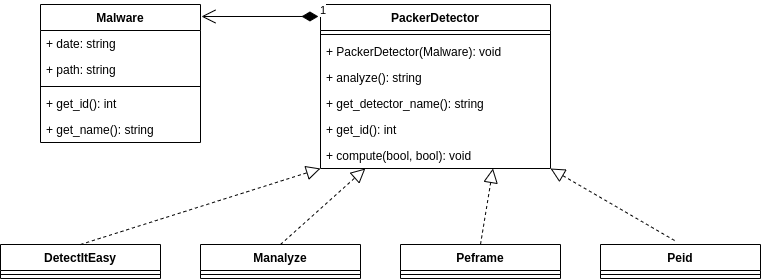
\includegraphics[width=\textwidth]{Figures/detector.png}
  \caption{Class diagram of our custom packer detector}
  \label{fig:Detector}
\end{figure}

PackerDetector's \texttt{compute()} method runs \texttt{analyze()} but accordingly to the provided options. With the \texttt{verbose} parameter set, the result of the analysis is displayed in the console while the \texttt{save} option actually stores the output in the database, introduced later in section \ref{gt}.

Here is a code snippet that will analyse the result of PEiD on a given malware. As one can notice, we chose Python as the programming language since it provides plenty of tools and API to easily manipulate tons of data.

\begin{lstlisting}[language=Python]
malware = Malware('20190615', 'malware/a0977e22deb6abde65a0cbfeb8949558')
peid = Peid(malware)
# There are 3 ways to display the result in the console
print(peid)
print(peid.analyze())
peid.compute(save=false, verbose=true)
\end{lstlisting}

We can then design a global \texttt{compute\_all()} method that will call every detector. Doing so allows to easily to add a new detector since it only requires to create its corresponding class that inherits from \texttt{PackerDetector}, and then append its call into the global method.

\begin{lstlisting}[language=Python]
def compute_all(malware):
    """ Displays the results of the four detectors and the new one just added."""
    Peid(malware).compute(false, true)
    Manalyze(malware).compute(false, true)
    Peframe(malware).compute(false, true)
    DetectItEasy(malware).compute(false, true)
    MyNewDetector(malware).compute(false, true)
\end{lstlisting}

With this structure in our hands, it is relatively easy to implement a script that quickly analyses every available malware without any overhead.